\begin{center}
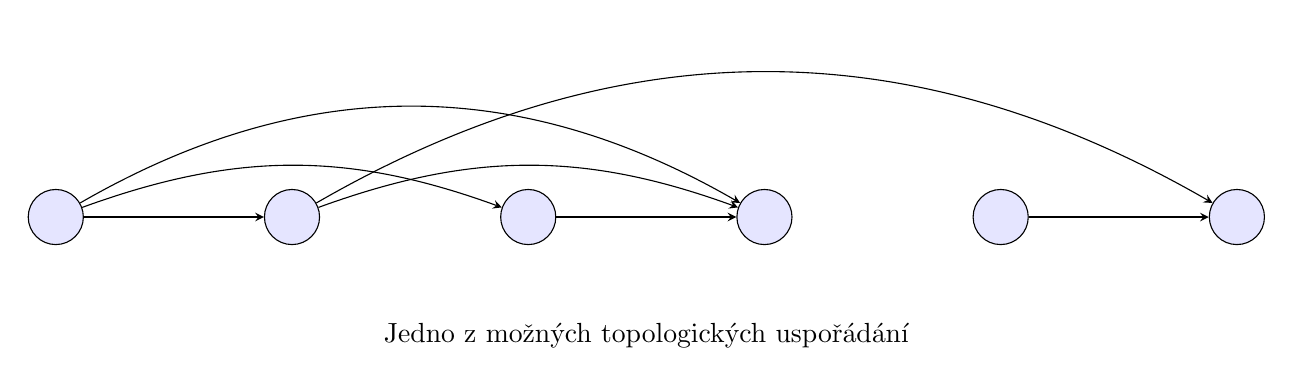
\begin{tikzpicture}[>=stealth,
    vnode/.style={circle, draw, minimum size=7mm, inner sep=0pt, fill=blue!10}]
  % Vertices placed horizontally
  \node[vnode] (a) at (0,0) {};
  \node[vnode] (b) at (3,0) {};
  \node[vnode] (c) at (6,0) {};
  \node[vnode] (d) at (9,0) {};
  \node[vnode] (e) at (12,0) {};
  \node[vnode] (f) at (15,0) {};

  % Directed edges (partial order)
  % Adjacent edges (now include all consecutive pairs)
  \draw[->] (a) -- (b);

  \draw[->] (c) -- (d);

  \draw[->] (e) -- (f);
  % Skipping edges (with bends to avoid intermediate vertices)
  \draw[->, bend left=20] (a) to (c);
  \draw[->, bend left=20] (b) to (d);
  \draw[->, bend left=30] (a) to (d);
  \draw[->, bend left=30] (b) to (f);

  % Topological ordering annotation centered below
  % Centered annotation below the whole diagram
  \node[align=center] at (7.5,-1.5) {Jedno z možných topologických uspořádání};
\end{tikzpicture}
\end{center}
